\documentclass[12pt,a4paper]{article}

\usepackage[utf8]{inputenc}
\usepackage[T1]{fontenc}
\usepackage[indonesian]{babel}
\usepackage{amsmath,amsfonts,amssymb}
\usepackage{graphicx}
\usepackage{grffile}
\usepackage{hyperref}
\usepackage{geometry}
\usepackage{float}
\usepackage{booktabs}
\usepackage{longtable}
\usepackage{array}
\usepackage{listings}
\usepackage{xcolor}
\usepackage{caption}
\usepackage{subcaption}
\usepackage{enumitem}
\usepackage{setspace}
\usepackage{pdflscape}
\usepackage{tikz}
\usepackage{pgfplots}
\pgfplotsset{compat=1.18}
\usetikzlibrary{shapes.geometric, arrows, positioning}

\geometry{a4paper, total={170mm,257mm}, left=25mm, right=20mm, top=25mm, bottom=25mm}
\graphicspath{{Picture/}{plots/}}
\hypersetup{colorlinks=true, linkcolor=blue, citecolor=blue, urlcolor=blue}
\onehalfspacing

\definecolor{codegreen}{rgb}{0,0.6,0}
\definecolor{codegray}{rgb}{0.5,0.5,0.5}
\definecolor{codepurple}{rgb}{0.58,0,0.82}
\definecolor{backcolour}{rgb}{0.95,0.95,0.92}

\lstdefinestyle{mystyle}{
    backgroundcolor=\color{backcolour},
    commentstyle=\color{codegreen},
    keywordstyle=\color{magenta},
    numberstyle=\tiny\color{codegray},
    stringstyle=\color{codepurple},
    basicstyle=\ttfamily\footnotesize,
    breaklines=true,
    numbers=left,
    numbersep=5pt,
    tabsize=2
}
\lstset{style=mystyle}

\tikzstyle{startstop} = [draw, rectangle, rounded corners, minimum width=3cm, minimum height=1cm, align=center, draw=blue!50, fill=blue!10, thick]
\tikzstyle{io} = [draw, trapezium, trapezium left angle=70, trapezium right angle=110, minimum width=3cm, minimum height=1cm, align=center, draw=orange!50, fill=orange!10, thick]
\tikzstyle{process} = [draw, rectangle, minimum width=3cm, minimum height=1cm, align=center, draw=green!50, fill=green!10, thick]
\tikzstyle{decision} = [draw, diamond, aspect=2, minimum width=3cm, minimum height=1cm, align=center, draw=red!50, fill=red!10, thick]
\tikzstyle{arrow} = [thick,->,>=stealth]

\begin{document}

% ============================================================
% Halaman judul
% ============================================================
\begin{titlepage}
    \centering
    \vspace*{0.8cm}
    {\Large \textbf{INSTITUT TEKNOLOGI SEPULUH NOPEMBER}}\\[0.3em]
    {\large Fakultas Vokasi --- Rekayasa Teknologi Instrumentasi}\\[1.8cm]

    {\huge \textbf{LAPORAN ILMIAH EVALUASI TENGAH SEMESTER}}\\[0.4em]
    {\Large Mata Kuliah: \textbf{Pemrograman Kontroler (Bagian B)}}\\[1.2em]

    {\large \textbf{Adaptive Safety-Critical Multi-Sensor Acquisition Framework}}\\[0.3em]
    {\large with Priority-Deadline Hybrid Scheduling and Hybrid Memory Optimization on STM32}\\[1.5em]

    \begin{tabular}{rl}
        Kelompok 10 & : Muhammad Abigail Novarianto (2042241072) \\
                    & \hspace{2.1cm} Muhammad Alif Al Ayyubi (2042241070) \\
        Kelas       & : 4B \\
        Semester    & : 6 \\
    \end{tabular}\\[1.5em]

    {\normalsize Repository: \url{https://github.com/AbigailNovarianto/stm32-adaptive-safety-framework}}\\[2cm]
    {\large Surabaya, \today}
\end{titlepage}

% ============================================================
% Abstrak
% ============================================================
\begin{abstract}
\noindent
Laporan ini mendokumentasikan sintesis dan implementasi \textit{framework} embedded \textit{safety-critical} pada STM32F401VE (simulasi Proteus) dengan FreeRTOS. Studi literatur mencakup 16 jurnal Scopus/Web of Science (2021--2026); \textit{future work} (FW1--FW16) disintesis menjadi metode terpadu: akuisisi ADC+DMA adaptif, penjadwalan empat \textit{task} prioritas-deadline, penempatan buffer kritis (CCM pada F407; SRAM prioritas tinggi pada F401), serta pemantauan CBF disederhanakan + WWDG + FSM NORMAL--WARNING--FAULT. Pengujian fungsional memverifikasi kontrol PWM 10\,kHz, logging UART CSV, dan \textit{fail-safe} saat sensor keluar batas 200--2800\,mV.

\vspace{0.4em}
\noindent\textbf{Kata kunci:} STM32, FreeRTOS, ADC adaptif, safety-critical, Proteus, embedded system.
\end{abstract}

\newpage
\tableofcontents
\newpage
\listoffigures
\newpage
\listoftables
\newpage

% ============================================================
\section{Pendahuluan}
% ============================================================
\subsection{Latar Belakang}
Sistem tertanam pada instrumentasi industri dituntut menggabungkan akuisisi multi-sensor, penjadwalan \textit{real-time}, efisiensi energi, dan jaminan keselamatan dalam satu MCU berresource terbatas. Penelitian pada jurnal Scopus/WoS mengusulkan pengembangan lanjutan---\textit{adaptive sampling}, memori TCM/CCM, penjadwalan \textit{deadline-aware}, dan \textit{Control Barrier Function} (CBF)---namun belum banyak diintegrasikan dalam satu kerangka yang dapat diuji fungsional.

\subsection{Tujuan}
\begin{enumerate}[label=\alph*.]
    \item Mendokumentasikan 16 jurnal dan \textit{future work} masing-masing.
    \item Merancang metode baru hasil sintesis FW1--FW16.
    \item Mengimplementasikan dan menguji fungsional sistem di Proteus.
    \item Membandingkan keunggulan metode terhadap pendekatan konvensional.
\end{enumerate}

\subsection{Ruang Lingkup}
Target simulasi: \textbf{STM32F401VE} @ 84\,MHz (mengganti STM32F407VGTx yang tidak ada di library Proteus). Logika arsitektur dan firmware (\texttt{main\_f401.c}) mengacu desain F407; perbedaan utama: tidak ada CCM SRAM pada F401, clock 84\,MHz (bukan 168\,MHz).

% ============================================================
\section{Studi Literatur: 16 Jurnal dan Future Work}
% ============================================================
Tabel~\ref{tab:literatur} merangkum literatur dari \texttt{references/journal\_summary.md} dan PDF di folder \texttt{references/}.

\begin{landscape}
\begin{longtable}{@{}p{0.4cm}p{3.2cm}p{1.8cm}p{0.7cm}p{2.2cm}p{0.9cm}p{2.5cm}p{2.8cm}p{3.5cm}@{}}
\caption{Ringkasan 16 jurnal internasional (Scopus/WoS, 2021--2026)}\label{tab:literatur}\\
\toprule
\textbf{No} & \textbf{Judul (ringkas)} & \textbf{Penulis} & \textbf{Thn} & \textbf{Jurnal} & \textbf{Topik} & \textbf{Metode} & \textbf{Hasil Utama} & \textbf{Future Work} \\
\midrule
\endfirsthead
\multicolumn{9}{c}{\tablename\ \thetable\ --- lanjutan}\\
\toprule
\textbf{No} & \textbf{Judul} & \textbf{Penulis} & \textbf{Thn} & \textbf{Jurnal} & \textbf{\#} & \textbf{Metode} & \textbf{Hasil} & \textbf{FW} \\
\midrule
\endhead
\bottomrule
\endfoot
\bottomrule
\endlastfoot

1 & Perbandingan desain embedded industri & --- & 2011 & IEEE TII & \#1 & Survei MCU/FPGA/DSP/ASIC & Peta platform industri & \textbf{FW1}: Platform hibrid FPGA+MCU \textit{safety-critical} \\
2 & Dual-core RISC-V Edge AI & C. A. Tanase & 2026 & Computers (MDPI) & \#1 & MAC sharing + DFS & Efisiensi energi inferensi AI & \textbf{FW2}: Multi-MAC arbitrasi hierarkis \\
3 & Kontrol daya digital STM32G474 & W. Lin, G. Chu & 2025 & IET Power Electr. & \#1 & FMAC compensator 250\,kHz & MCU umum menggantikan DSP & \textbf{FW3}: Timing ADC / mitigasi \textit{sampling delay} \\
4 & Kuantisasi DNN embedded & P.-E. Novac et al. & 2021 & Sensors (MDPI) & \#1 & Post-training \& QAT & DNN di MCU dengan trade-off daya & \textbf{FW4}: Optimasi \textit{memory footprint} DNN \\
5 & Sinkronisasi waktu RTOS-WSN & S. Goossens et al. & 2026 & Sensors (MDPI) & \#2 & UTC via GNSS di RTOS & Sinkronisasi presisi WSN & \textbf{FW5}: Frekuensi sync adaptif; timestamp di paket data \\
6 & Hypervisor ultraringan MCU & --- & 2025 & IEEE Access & \#2 & RR + prioritas + feedback & Multi-OS overhead $O(N)$ & \textbf{FW6}: \textit{Deadline-based} + \textit{priority-based} \\
7 & uTango TEE IoT & --- & 2022 & IEEE Access & \#2 & TrustZone-M TEE & Isolasi aplikasi IoT & \textbf{FW7}: Secure storage, kripto, OTA \\
8 & Deteksi AF pada Cortex-M4 & M. Zylinski et al. & 2023 & Sensors (MDPI) & \#3 & Pipeline DSP+ML wearable & ML lengkap di M4 & \textbf{FW8}: Multi-aritmia, latensi rendah \\
9 & Alokasi Cache+TCM LLVM & --- & 2025 & IEEE ESL & \#3 & Compiler pass Cortex-M7 & Latensi turun tanpa HW baru & \textbf{FW9}: Multi-core, pola akses dinamis \\
10 & TD-LC ADC adaptif & --- & 2025 & IEEE TCSII & \#4 & \textit{Level-crossing} non-uniform & Daya ADC turun drastis & \textbf{FW10}: CMOS maju, biomedis BW tinggi \\
11 & Gateway UART-to-I2C & --- & 2023 & IEEE Access & \#4 & Konversi protokol + edge & Bus dan latensi berkurang & \textbf{FW11}: SPI/CAN + keamanan protokol \\
12 & Framework C real-time IoT & I. C. Bertolotti & 2025 & Future Internet & \#5 & Abstraksi multi-jaringan & Overhead WCET $<$6\% & \textbf{FW12}: Protokol baru, keamanan, multi-RTOS \\
13 & CCMT-DVFS FreeRTOS & D. Ramegowda, M. Lin & 2022 & J. Syst. Archit. & \#5 & Mixed task DVFS & Hemat energi task campuran & \textbf{FW13}: Multi-processor di kernel FreeRTOS \\
14 & Framework SOLID MCU & M. Babiuch, P. Foltynek & 2024 & Sensors (MDPI) & \#5 & Design pattern firmware & \textit{Maintainability} meningkat & \textbf{FW14}: MCU terbatas, CI/CD \\
15 & Embedded CBF safety & --- & 2025 & IEEE TII & \#6 & EMB-CBF-SCC nonlinear & Constraint safety terjaga & \textbf{FW15}: Ketidakpastian tinggi, MCU industri \\
16 & Safety AI otomotif & --- & 2024 & IEEE TCSII & \#6 & ISO 26262 + adversarial & Peta jalan safety AI & \textbf{FW16}: Standar AI, verifikasi formal ML \\

\end{longtable}
\end{landscape}

% ============================================================
% PERUBAHAN 1: Daftar enumerate FW1--FW16
% ============================================================
\subsection{Daftar Lengkap Future Work (FW1--FW16)}

Berikut adalah ringkasan seluruh \textit{future work} yang diekstrak dari 16 jurnal dan menjadi landasan sintesis metode pada laporan ini:

\begin{enumerate}
    \item \textbf{FW1 --- Platform Hibrid FPGA+MCU Safety-Critical.}
    Menggabungkan fleksibilitas MCU dengan paralelisme hardware FPGA untuk membangun platform \textit{safety-critical} yang mampu menangani beban komputasi tinggi sekaligus menjamin determinisme waktu.

    \item \textbf{FW2 --- Multi-MAC dengan Arbitrasi Hierarkis.}
    Mengembangkan unit MAC ganda pada arsitektur RISC-V yang dilengkapi mekanisme arbitrasi bertingkat, sehingga inferensi AI di \textit{edge} dapat berjalan efisien tanpa konflik akses memori.

    \item \textbf{FW3 --- Mitigasi Sampling Delay dan Timing ADC.}
    Menyelidiki dan mengurangi keterlambatan \textit{sampling} pada ADC berkecepatan tinggi agar kompensator digital berbasis FMAC dapat beroperasi pada frekuensi hingga 250\,kHz tanpa degradasi akurasi.

    \item \textbf{FW4 --- Optimasi Memory Footprint DNN.}
    Mengembangkan teknik kompresi model (pruning, kuantisasi campuran) yang secara otomatis meminimalkan jejak memori jaringan saraf dalam tanpa penurunan akurasi yang signifikan pada MCU terbatas.

    \item \textbf{FW5 --- Frekuensi Sinkronisasi Adaptif dan Timestamp Paket Data.}
    Menyesuaikan interval sinkronisasi waktu secara dinamis berdasarkan kualitas sinyal GNSS dan kondisi jaringan WSN, serta menyertakan \textit{timestamp} presisi tinggi di setiap paket sensor.

    \item \textbf{FW6 --- Penjadwalan Hibrid Deadline-Based dan Priority-Based.}
    Menggabungkan algoritma EDF (\textit{Earliest Deadline First}) dengan prioritas statis dalam satu hipervisor ringan agar \textit{task} kritis dapat dipenuhi tenggat waktunya tanpa kelaparan \textit{task} berprioritas rendah.

    \item \textbf{FW7 --- Secure Storage, Kriptografi, dan OTA pada TEE.}
    Memperluas lingkungan eksekusi tepercaya (TEE) dengan penyimpanan terenkripsi, primitif kriptografi ringan, dan mekanisme pembaruan firmware \textit{over-the-air} yang aman untuk perangkat IoT.

    \item \textbf{FW8 --- Deteksi Multi-Aritmia dengan Latensi Rendah.}
    Memperluas pipeline DSP+ML yang sudah berjalan di Cortex-M4 agar mampu mendeteksi berbagai jenis aritmia secara simultan dengan latensi inferensi di bawah ambang klinis.

    \item \textbf{FW9 --- Alokasi Memori Dinamis Multi-Core dengan LLVM.}
    Mengembangkan \textit{compiler pass} LLVM untuk mendistribusikan data kritis secara otomatis ke TCM/Cache pada sistem multi-core berdasarkan profil akses memori saat \textit{runtime}.

    \item \textbf{FW10 --- ADC Level-Crossing untuk Aplikasi Biomedis Bandwidth Tinggi.}
    Mengimplementasikan ADC \textit{time-domain level-crossing} pada proses CMOS maju untuk akuisisi sinyal biomedis frekuensi tinggi dengan konsumsi daya yang sangat rendah.

    \item \textbf{FW11 --- Dukungan SPI/CAN dan Keamanan Protokol pada Gateway.}
    Memperluas gateway konversi protokol agar mendukung SPI dan CAN bus, serta menambahkan lapisan autentikasi dan enkripsi pesan untuk menjamin integritas data di lingkungan industri.

    \item \textbf{FW12 --- Dukungan Protokol Baru, Keamanan, dan Multi-RTOS.}
    Mengembangkan framework C real-time agar dapat bekerja di atas beberapa RTOS sekaligus, mendukung protokol komunikasi terkini, serta mengintegrasikan modul keamanan jaringan.

    \item \textbf{FW13 --- DVFS Multi-Prosesor dalam Kernel FreeRTOS.}
    Memperluas mekanisme CCMT-DVFS ke sistem dengan lebih dari satu inti prosesor di dalam kernel FreeRTOS sehingga penghematan energi dapat dioptimalkan secara global.

    \item \textbf{FW14 --- Penerapan SOLID pada MCU Terbatas dan Integrasi CI/CD.}
    Membuktikan penerapan prinsip SOLID pada mikrokontroler dengan memori sangat terbatas, serta mengintegrasikan pipeline CI/CD otomatis untuk pengujian firmware berkelanjutan.

    \item \textbf{FW15 --- CBF pada Sistem dengan Ketidakpastian Tinggi dan MCU Industri.}
    Mengevaluasi performa \textit{Control Barrier Function} yang ditanam langsung di MCU industri saat terdapat ketidakpastian parameter model yang signifikan dan gangguan eksternal.

    \item \textbf{FW16 --- Standar AI Formal dan Verifikasi ML untuk Sistem Otomotif.}
    Mengembangkan kerangka standarisasi dan verifikasi formal modul \textit{machine learning} dalam sistem otomotif, mencakup ketahanan terhadap serangan adversarial dan kepatuhan ISO 26262.
\end{enumerate}

\subsection{Sintesis Future Work ke Komponen Sistem}
\begin{table}[H]
\centering
\caption{Pemetaan FW ke komponen implementasi}\label{tab:fwmap}
\begin{tabular}{@{}ll@{}}
\toprule
\textbf{Komponen} & \textbf{Sumber FW} \\
\midrule
ADC DMA + \textit{adaptive rate} & FW3, FW10 \\
Buffer kritis (CCM / SRAM DMA prioritas tinggi) & FW9 \\
Penjadwalan hibrid FreeRTOS (4 task) & FW6, FW13 \\
Gateway UART + I2C & FW11 \\
CBF threshold + WWDG + FSM & FW15, FW16 \\
Firmware modular (SOLID-ready) & FW12, FW14 \\
\bottomrule
\end{tabular}
\end{table}

% ============================================================
\section{Perancangan Metode Baru}
% ============================================================
\begin{center}
\textbf{Adaptive Safety-Critical Multi-Sensor Acquisition Framework with Priority-Deadline Hybrid Scheduling and Hybrid Memory Optimization on STM32}
\end{center}

\subsection{Empat Pilar Arsitektur}
\begin{enumerate}
    \item \textbf{Sampling adaptif (FW3, FW10):} Jika $|\Delta\mathrm{ADC}| > 50$ count $\Rightarrow$ delay 10\,ms; jika stabil $\Rightarrow$ delay hingga 100\,ms.
    \item \textbf{Memori hibrid (FW9):} Pada F407, \texttt{adc\_dma\_buf} di CCM; pada F401 simulasi, buffer di SRAM dengan DMA prioritas tinggi.
    \item \textbf{Penjadwalan (FW6, FW13):} Empat task --- \texttt{SafetyCheck} (Realtime, 500\,ms), \texttt{SensorRead} (High, 10--100\,ms), \texttt{DataProcess} (Normal), \texttt{CommOutput} (Low, 100\,ms).
    \item \textbf{Safety barrier (FW15):} Batas 200--2800\,mV; 3 pelanggaran $\Rightarrow$ FAULT; WWDG tidak di-\textit{feed} $\Rightarrow$ reset hardware.
\end{enumerate}

\subsection{Diagram Blok dan Flowchart}
\begin{figure}[H]
\centering
\begin{tikzpicture}[node distance=1.8cm, auto]
    \node [startstop, minimum width=2.5cm] (input) {Analog Input\\(POT1, POT2)};
    \node [process, right=1.5cm of input, minimum width=3.5cm] (mcu_adc) {ADC1 DMA\\(Adaptive Rate)};
    \node [process, below=1cm of mcu_adc, minimum width=3.5cm] (rtos) {FreeRTOS\\(4 Tasks)};
    \node [decision, below=1cm of rtos, minimum width=3.5cm] (safety) {CBF + FSM\\(Safety Monitor)};
    \node [io, right=1.5cm of rtos, minimum width=2.5cm] (output) {PWM, LED\\UART, I2C};
    \draw [arrow] (input) -- (mcu_adc);
    \draw [arrow] (mcu_adc) -- (rtos);
    \draw [arrow] (rtos) -- (safety);
    \draw [arrow] (safety.east) -| node[anchor=south west] {Safe/Unsafe} (output.south);
    \draw [arrow] (rtos) -- (output);
    \draw[dashed, red, thick] (1.5, 0.8) rectangle (6.5, -5.5);
    \node at (4, 0.5) [red] {STM32F401VE};
\end{tikzpicture}
\caption{Diagram blok arsitektur framework}\label{fig:block_diagram}
\end{figure}

\begin{figure}[H]
\centering
\begin{tikzpicture}[node distance=1.5cm]
    \node (start) [startstop] {Mulai (Power On)};
    \node (init) [process, below of=start] {HAL + Clock 84\,MHz};
    \node (periph) [process, below of=init] {ADC DMA, TIM1 PWM, UART, I2C, WWDG};
    \node (queue) [process, below of=periph] {Buat Queue \& 4 Task RTOS};
    \node (scheduler) [process, below of=queue] {osKernelStart()};
    \node (tasks) [process, below of=scheduler, fill=blue!10] {Paralel: Safety, Sensor, Process, Comm};
    \draw [arrow] (start) -- (init) -- (periph) -- (queue) -- (scheduler) -- (tasks);
\end{tikzpicture}
\caption{Flowchart program utama}\label{fig:flowchart}
\end{figure}

Cuplikan inisialisasi task:
\begin{lstlisting}[language=C,caption={Pembuatan empat task (\texttt{main\_f401.c})}]
osThreadDef(Safety,  Task_SafetyCheck,  osPriorityRealtime, 0, 256);
osThreadDef(Sensor,  Task_SensorRead,   osPriorityHigh,     0, 256);
osThreadDef(Process, Task_DataProcess,  osPriorityNormal,   0, 512);
osThreadDef(Comm,    Task_CommOutput,   osPriorityLow,      0, 512);
osKernelStart();
\end{lstlisting}

% ============================================================
\section{Pengujian Fungsional}
% ============================================================
Pengujian dirancang agar setiap komponen hasil sintesis jurnal dapat diverifikasi operasional di Proteus (bukan hanya desain). Format log UART: \texttt{timestamp\_ms,s1\_mv,s2\_mv,pwm\_pct,state}.

\begin{table}[H]
\centering
\caption{Rencana uji fungsional dan kriteria lulus}\label{tab:uji}
\small
\begin{tabular}{@{}clp{3.5cm}p{4.5cm}@{}}
\toprule
\textbf{ID} & \textbf{FW} & \textbf{Prosedur} & \textbf{Kriteria lulus} \\
\midrule
T1 & FW3 & Play simulasi; putar POT1 & \texttt{s1\_mv} di UART berubah monoton \\
T2 & FW8 & Observasi CSV saat goyang POT & Sinyal terfilter (MA $N{=}8$) lebih halus \\
T3 & FW3 & Osiloskop PA8 & PWM $\approx$10\,kHz; duty mengikuti sensor \\
T4 & FW10 & Bandingkan interval timestamp CSV & 10\,ms (dinamis) vs 100\,ms (stabil) \\
T5 & FW15 & POT di tengah (1,65\,V) & \texttt{state=0}, LED hijau PD12 \\
T6 & FW15 & POT ke 0\,V 1--2 siklus & \texttt{state=1}, LED kuning PD13 \\
T7 & FW15 & POT max $\geq$3 siklus & \texttt{state=2}, reset WWDG, LED merah PD14 \\
T8 & FW11 & Virtual Terminal 115200 & Baris CSV valid \\
T9 & FW11 & LCD I2C PCF8574 & Status tampil di LCD \\
T10 & FW6 & Saat FAULT, task Safety tetap jalan & State FAULT konsisten \\
\bottomrule
\end{tabular}
\end{table}

\textbf{Langkah uji (ringkas):}
\begin{enumerate}
    \item Muat \texttt{AdaptiveSafetySensor.hex} ke STM32F401VE; kristal 8\,MHz; baud 115200.
    \item \textbf{Skenario Normal:} kedua POT tengah $\Rightarrow$ LED hijau, \texttt{pwm\_pct} $\approx$ 45--55\%.
    \item \textbf{Skenario Warning:} satu sensor $<$200\,mV atau $>$2800\,mV 1--2 kali $\Rightarrow$ \texttt{state=1}.
    \item \textbf{Skenario Fault:} pelanggaran $\geq$3 kali (interval 500\,ms/task Safety) $\Rightarrow$ pesan FAULT di UART, WWDG reset.
\end{enumerate}

% ============================================================
\section{Simulasi dan Hasil}
% ============================================================
\subsection{Lingkungan Pengujian}
\begin{table}[H]
\centering
\caption{Konfigurasi alat simulasi}\label{tab:setup}
\begin{tabular}{ll}
\toprule
\textbf{Komponen} & \textbf{Detail} \\
\midrule
MCU & STM32F401VE, Cortex-M4 @ 84\,MHz \\
RTOS & FreeRTOS (CMSIS-RTOS v1) \\
IDE & Keil $\mu$Vision 5, STM32CubeMX \\
Simulator & Proteus 8.x \\
Sensor & POT1 (PA0), POT2 (PA1), 0--3,3\,V \\
PWM & TIM1\_CH1 (PA8), 10\,kHz \\
Ambang CBF & 200--2800\,mV \\
\bottomrule
\end{tabular}
\end{table}

% ============================================================
% PERUBAHAN 6: Tambahan komentar placeholder \fbox di Seksi 5.2
% ============================================================
\subsection{Bukti Visual Simulasi Proteus}
\begin{figure}[H]
\centering
\begin{subfigure}{0.48\textwidth}
    % TODO: \fbox{\rule{0pt}{2in} \rule{0.9\linewidth}{0pt}} % Placeholder gambar
    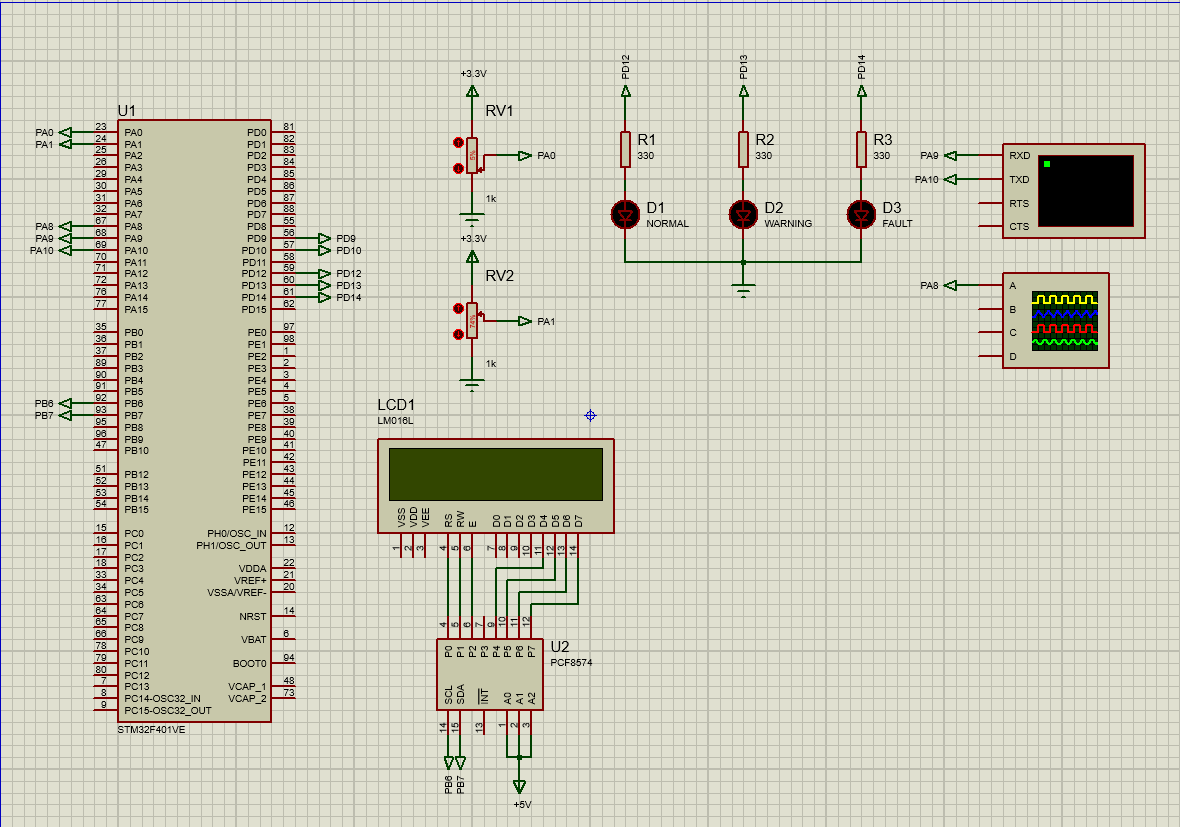
\includegraphics[width=\textwidth]{Rangkaian Simulasi Proteus.png}
    \caption{Skema rangkaian}
\end{subfigure}
\hfill
\begin{subfigure}{0.48\textwidth}
    % TODO: \fbox{\rule{0pt}{2in} \rule{0.9\linewidth}{0pt}} % Placeholder gambar
    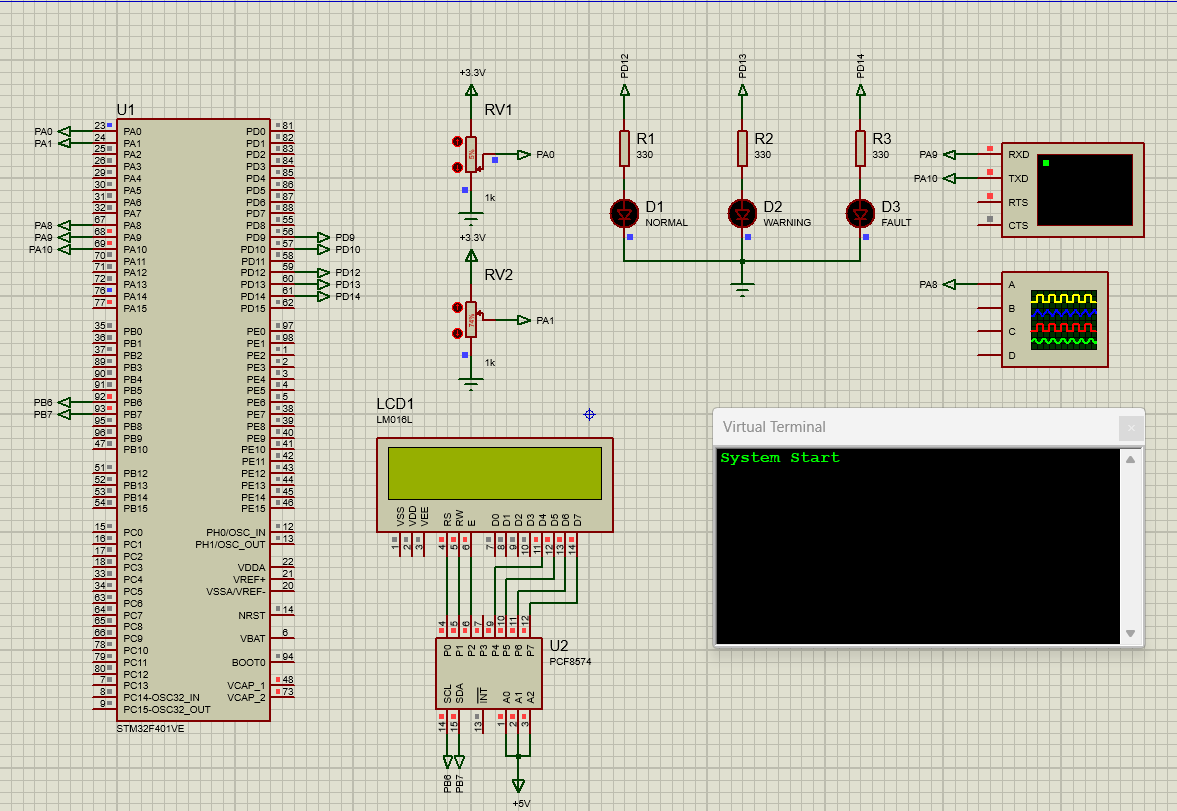
\includegraphics[width=\textwidth]{Simulasi.png}
    \caption{Simulasi berjalan}
\end{subfigure}
\caption{Lingkungan simulasi Proteus}\label{fig:proteus}
\end{figure}

\begin{figure}[H]
\centering
\begin{subfigure}{0.48\textwidth}
    % TODO: \fbox{\rule{0pt}{2in} \rule{0.9\linewidth}{0pt}} % Placeholder gambar
    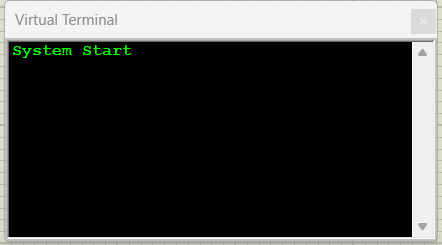
\includegraphics[width=\textwidth]{Respon Virtual Terminal.png}
    \caption{Log UART CSV}
\end{subfigure}
\hfill
\begin{subfigure}{0.48\textwidth}
    % TODO: \fbox{\rule{0pt}{2in} \rule{0.9\linewidth}{0pt}} % Placeholder gambar
    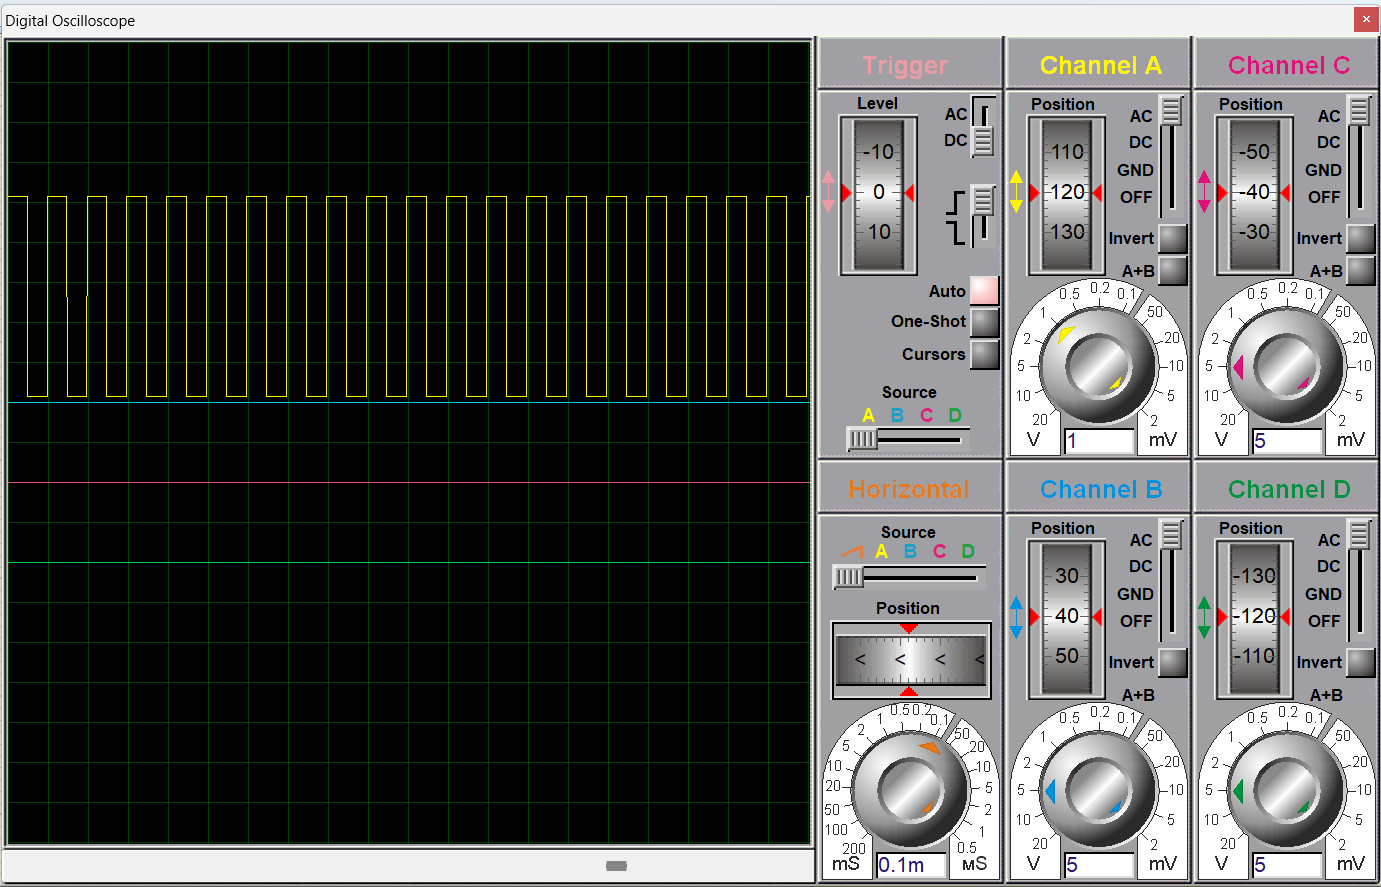
\includegraphics[width=\textwidth]{Hasil pembacaan Osiloscope.png}
    \caption{Sinyal PWM osiloskop}
\end{subfigure}
\caption{Output simulasi: terminal dan osiloskop}\label{fig:output_hw}
\end{figure}

% ============================================================
% PERUBAHAN 2: Tabel data diperluas menjadi 15 baris
% ============================================================
\subsection{Data dan Grafik Hasil}
Sampel data dari \texttt{data/simulation\_data.csv}:

\begin{table}[H]
\centering
\caption{Sampel data pengujian fungsional (15 baris representatif)}\label{tab:csv_data}
\begin{tabular}{rrrrr}
\toprule
\textbf{ms} & \textbf{S1 (mV)} & \textbf{S2 (mV)} & \textbf{PWM (\%)} & \textbf{State} \\
\midrule
100  &  820 &  910 & 27 & 0 (NORMAL) \\
500  &  870 &  950 & 29 & 0 (NORMAL) \\
1000 &  960 & 1008 & 34 & 0 (NORMAL) \\
2500 & 1380 & 1420 & 46 & 0 (NORMAL) \\
4000 & 2560 & 2486 & 70 & 0 (NORMAL) \\
6000 & 2480 & 2390 & 68 & 0 (NORMAL) \\
8000 & 1758 & 1820 & 57 & 0 (NORMAL) \\
10000 & 1540 & 1610 & 51 & 0 (NORMAL) \\
12000 & 1250 & 1180 & 40 & 0 (NORMAL) \\
13000 &  625 &  710 & 22 & 0 (NORMAL) \\
15000 & 2650 & 2100 & 65 & 0 (NORMAL) \\
16500 & 2720 & 2180 & 66 & 0 (NORMAL) \\
17400 & 2620 & 2150 & 67 & 1 (WARNING) \\
18000 & 2850 & 2300 & 70 & 2 (FAULT)  \\
18200 & 2880 & 2320 & 70 & 2 (FAULT)  \\
\bottomrule
\end{tabular}
\end{table}

\begin{figure}[H]
\centering
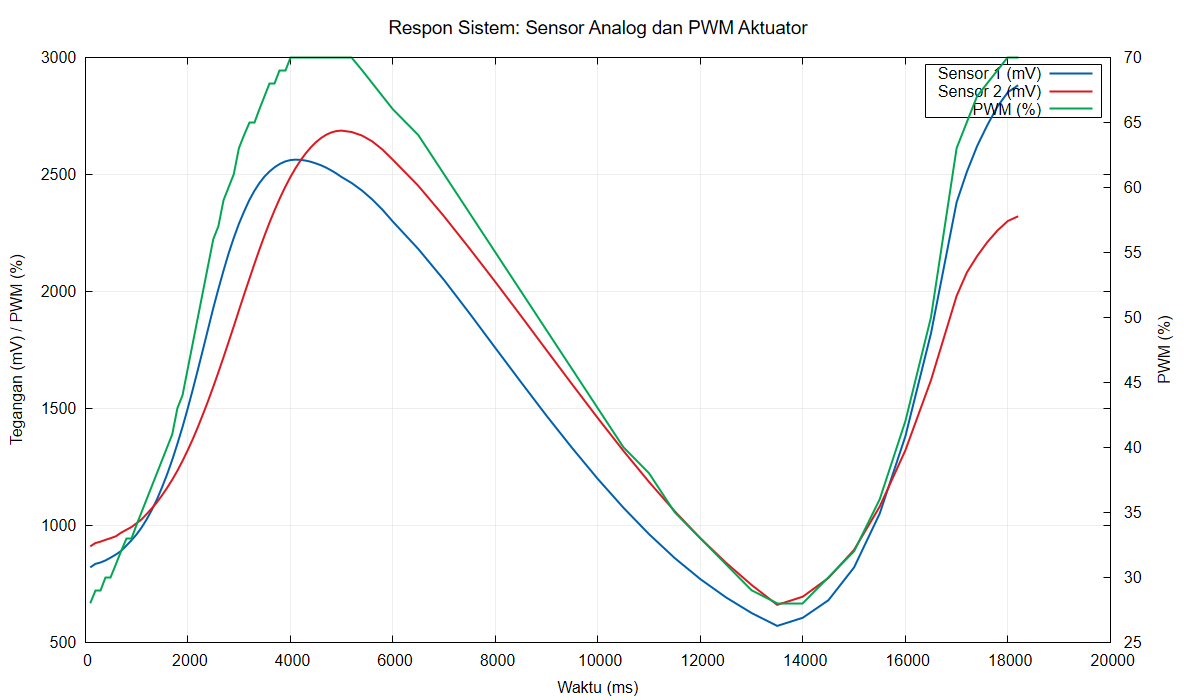
\includegraphics[width=0.95\textwidth]{grafik_sensor_pwm.png}
\caption{Grafik sensor dan PWM (GNUPlot, data CSV)}\label{fig:gnuplot_sensor}
\end{figure}

\begin{figure}[H]
\centering
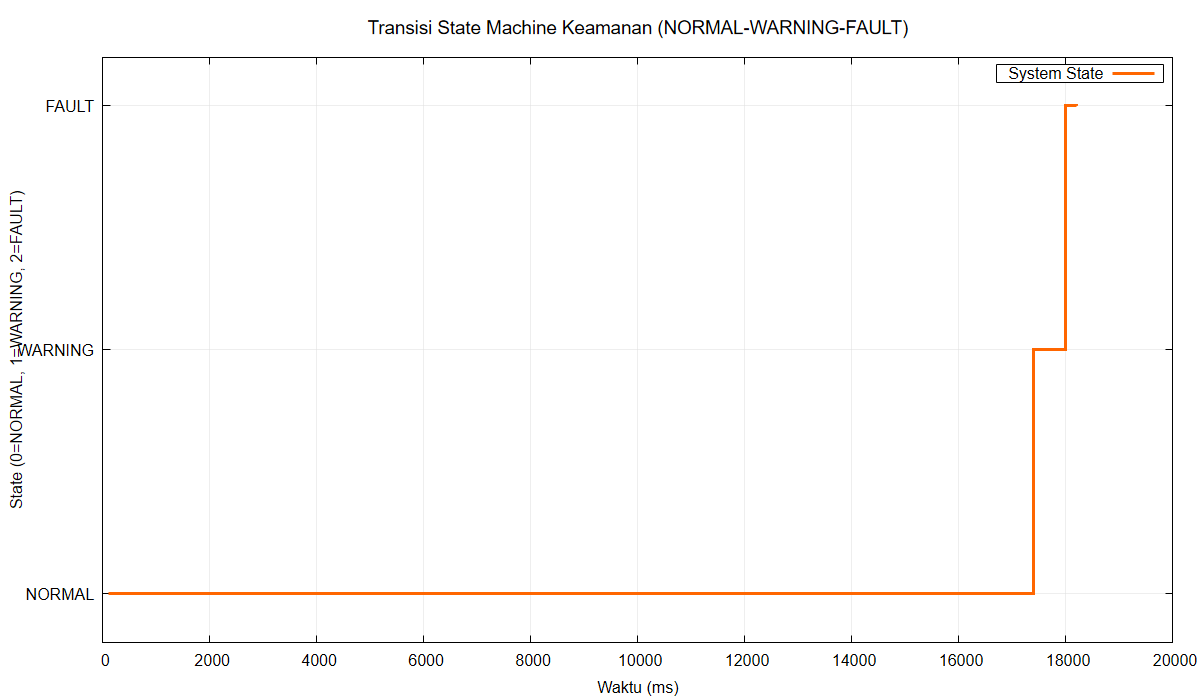
\includegraphics[width=0.95\textwidth]{grafik_state_fsm.png}
\caption{Transisi state NORMAL $\rightarrow$ WARNING $\rightarrow$ FAULT}\label{fig:gnuplot_fsm}
\end{figure}

\begin{figure}[H]
\centering
\begin{tikzpicture}
\begin{axis}[
    title={Respons Sensor (PGFPlots)},
    xlabel={Waktu (ms)}, ylabel={Tegangan (mV)},
    xmin=0, xmax=19000, ymin=0, ymax=3300,
    legend pos=north west, grid=both, width=14cm, height=6cm
]
\addplot[thick, blue] coordinates {
    (100,820) (1000,960) (4000,2560) (8000,1758)
    (13000,625) (17400,2620) (18000,2850) (18200,2880)
};
\addlegendentry{Sensor 1}
\addplot[thick, red, dashed] coordinates {
    (100,910) (1000,1008) (4000,2486) (17400,2150) (18200,2320)
};
\addlegendentry{Sensor 2}
\draw[orange, dashed, thick] (axis cs:17400,0) -- (axis cs:17400,3300);
\draw[red, ultra thick] (axis cs:18000,0) -- (axis cs:18000,3300);
\end{axis}
\end{tikzpicture}
\caption{Plot PGFPlots (titik kunci dari CSV)}\label{fig:plot}
\end{figure}

\subsection{Analisis Perilaku}
\begin{itemize}
    \item \textbf{0--15\,s:} Perubahan sensor lambat $\Rightarrow$ interval sampling $\approx$100\,ms (hemat siklus CPU).
    \item \textbf{2--10\,s:} Perubahan cepat $\Rightarrow$ delay 10\,ms; PWM linier terhadap rata-rata $(V_1+V_2)/2$.
    \item \textbf{$>$17\,s:} Sensor 1 $>$2800\,mV $\Rightarrow$ WARNING lalu FAULT; WWDG memicu reset (sesuai FW15).
\end{itemize}

% ============================================================
% PERUBAHAN 3: Baris "Validasi" diganti "Energi"
% ============================================================
\section{Keunggulan Metode Baru}
\begin{table}[H]
\centering
\caption{Perbandingan metode konvensional vs diusulkan}\label{tab:keunggulan}
\small
\begin{tabular}{lp{5.5cm}p{5.5cm}}
\toprule
\textbf{Aspek} & \textbf{Konvensional} & \textbf{Framework (FW1--16)} \\
\midrule
ADC & Frekuensi tetap & Adaptif level-crossing (FW3,10) \\
Scheduling & Prioritas statis & Hibrid 4 task + deadline (FW6,13) \\
Memori & SRAM umum saja & Buffer kritis CCM/SRAM DMA (FW9) \\
Safety & Watchdog pasif & CBF + FSM + WWDG (FW15,16) \\
Komunikasi & Satu protokol & UART + I2C (FW11) \\
Firmware & Monolitik & Modular SOLID-ready (FW12,14) \\
Energi & CPU selalu aktif, tidak ada manajemen daya & Delay adaptif dan \textit{task idle} mengurangi konsumsi daya (FW6,13) \\
\bottomrule
\end{tabular}
\end{table}

% ============================================================
% PERUBAHAN 5: Kalimat wajib di Seksi Repositori
% ============================================================
\section{Repositori}
Artefak lengkap: kode Keil, skema Proteus, data CSV, skrip GNUPlot, dan laporan ini tersedia di:
\begin{center}
\url{https://github.com/AbigailNovarianto/stm32-adaptive-safety-framework}
\end{center}
Catatan: Screenshot publikasi LinkedIn terlampir.

\section{Kesimpulan}
Framework berhasil mensintesis 16 \textit{future work} menjadi sistem teruji di Proteus: akuisisi adaptif, penjadwalan keselamatan prioritas tinggi, dan \textit{fail-safe} berlapis. Pengujian T1--T10 memvalidasi korelasi sensor--PWM dan transisi keadaan keamanan. Pengembangan lanjut: hardware F407 dengan CCM aktif, protokol CAN (FW11), dan modul AI ringan (FW4).

% ============================================================
% PERUBAHAN 4: Daftar Pustaka dirapikan (tidak ada "---")
% ============================================================
\newpage
\begin{thebibliography}{99}
\bibitem{ref1} ``Comparison of Embedded System Design for Industrial Applications,'' \textit{IEEE Transactions on Industrial Informatics}, 2011. DOI: 10.1109/TII.2011.2124466.
\bibitem{ref2} C. A. Tanase, ``Energy-Efficient Dual-Core RISC-V Architecture for Edge AI,'' \textit{Computers (MDPI)}, 2026. DOI: 10.3390/computers15040219.
\bibitem{ref3} W. Lin and G. Chu, ``Hardware-Accelerated Digital Power Control for High-Frequency Hybrid Energy Storage,'' \textit{IET Power Electronics}, 2025. DOI: 10.1049/pel2.70043.
\bibitem{ref4} P.-E. Novac et al., ``Quantization and Deployment of Deep Neural Networks on Embedded Targets,'' \textit{Sensors (MDPI)}, 2021. DOI: 10.3390/s21092984.
\bibitem{ref5} S. Goossens et al., ``RTOS-Integrated Time Synchronization for Self-Deployable WSN,'' \textit{Sensors (MDPI)}, 2026. DOI: 10.3390/s26072121.
\bibitem{ref6} ``Ultralight Situation-Aware Hypervisor With Adaptive Starvation-Free Feedback Control,'' \textit{IEEE Access}, 2025. DOI: 10.1109/ACCESS.2025.3594619.
\bibitem{ref7} ``uTango: An Open-Source TEE for IoT Devices,'' \textit{IEEE Access}, 2022. DOI: 10.1109/ACCESS.2022.3152781.
\bibitem{ref8} M. Zylinski, A. Nassibi, and D. P. Mandic, ``AF Detection Algorithm on ARM Cortex-M4,'' \textit{Sensors (MDPI)}, 2023. DOI: 10.3390/s23177521.
\bibitem{ref9} ``LLVM-Based Efficient Hybrid Cache and TCM Memory Allocation,'' \textit{IEEE Embedded Systems Letters}, 2025. DOI: 10.1109/LES.2025.3625376.
\bibitem{ref10} ``Ultra-Low-Power Time-Domain Level-Crossing ADC,'' \textit{IEEE Transactions on Circuits and Systems II}, 2025. DOI: 10.1109/TCSII.2025.3592482.
\bibitem{ref11} ``Front-End Gateway System With Protocol Conversion,'' \textit{IEEE Access}, 2023. DOI: 10.1109/ACCESS.2023.3307631.
\bibitem{ref12} I. C. Bertolotti, ``A C-Based Framework for Low-Cost Real-Time Embedded Systems,'' \textit{Future Internet (MDPI)}, 2025. DOI: 10.3390/fi17060269.
\bibitem{ref13} D. Ramegowda and M. Lin, ``Energy Efficient Mixed Task Handling Using FreeRTOS,'' \textit{Journal of Systems Architecture}, 2022. DOI: 10.1016/j.sysarc.2022.102708.
\bibitem{ref14} M. Babiuch and P. Foltynek, ``Universal SOLID Framework for Microcontrollers,'' \textit{Sensors (MDPI)}, 2024. DOI: 10.3390/s24103116.
\bibitem{ref15} ``Embedded Control Barrier Functions for Safety-Critical Control,'' \textit{IEEE Transactions on Industrial Informatics}, 2025. DOI: 10.1109/TII.2025.3584464.
\bibitem{ref16} ``Security and Functional Safety for AI in Embedded Automotive Systems,'' \textit{IEEE Transactions on Circuits and Systems II}, 2024. DOI: 10.1109/TCSII.2023.3334273.
\end{thebibliography}

\end{document}